
%%%%%%%%%%%%%%%%%%%%%%%%%%%%%%%%%%%%%%%%%%%%%%%%%%%%%%%%%%%%%
%% HEADER
%%%%%%%%%%%%%%%%%%%%%%%%%%%%%%%%%%%%%%%%%%%%%%%%%%%%%%%%%%%%%

\documentclass[a4paper, onecolumn, oneside, 11pt]{article}
\usepackage{cmbright}
\usepackage[T1]{fontenc}
\usepackage[english]{babel}

%\usepackage[dvips]{graphics} %%graphics and normal LaTeX
%\usepackage{amsmath}
%\usepackage{amsthm}
%\usepackage{amsfonts}
\usepackage{amssymb}
\usepackage{graphicx}
\usepackage{rotating}
\usepackage{pdflscape}
\usepackage{abstract}
\usepackage[ table ]{ xcolor }
\usepackage[square, comma, sort&compress, longnamesfirst]{natbib} %
\usepackage{subfigure}
\usepackage{setspace}
%\singlespacing %% 1-spacing (default)s
%\onehalfspacing

%%% END Article customizations

%%% The "real" document content comes below...

\title{Saccadic Biases}

\author{Alasdair D. F. Clarke, Matthew J. Stainer}


%\date{} % Activate to display a given date or no date (if empty),

% otherwise the current date is printed

\begin{document}

\maketitle

\begin{abstract}
More bias modelling! Cause who can be bothered running actual experiments?

HERE IS SOME STUFF TO SEE IF I EXIST!
\end{abstract}


\section{Introduction}

Improve on last year's \citep{clarke-tatler2014} effort. More sophisticated biases. And some examples of how to use biases for improved data analysis. 

\section{Methods}

\subsection{Datasets}

\subsection{Pre-processing}
Generally, there are some things we want to consider:
\begin{itemize}
\item Normalise fixation positions relative to image frame. 
\item Boot-strapping? 
\item Merge datasets or model individually? 
\item Remove intial fixation? (from all analysis??)
\end{itemize} 

And specifically for the Flow analysis, there are some further things we may want to do:
\begin{itemize}
\item What about trasforming the data so that it is unbounded: $x'=\frac{x}{1-x}$?
\item Mirroring the data (where relevant)... left = right and up = down?
\end{itemize} 

\section{Biases}

We will model and discuss saccadic flow, coarse-to-fine, and left v right. 

\subsection{Saccadic Flow}

Saccadic flow can be thought of as a generalisation of the central bias. Instead of computing the distribution of all saccadic endpoints in a dataset, we look at the distribution of saccade endpoints given the start points. So for a saccade from $(x_0, y_0)$ to $(x_1, y1)$ we want to model $p(x_1,y_1|x_0, y0)$ This is illustrated in \ref{fig:exampleSaccadic Flow}.



\begin{figure}
[insert example image here]
\caption{Empirical example of saccadic flow from blah dataset.}
\label{fig:exampleSaccadic Flow}
\end{figure}

\subsubsection{Modelling}

We will model saccadic flow using multivariate skew-$t$ distributions \citep{azzalini2015}. The multivariate skew-normal distribution \citep{azzalini1996} is given by:

\begin{equation}
\phi(z; \lambda) = 2\phi(z)\Phi(\lambda z) 
\end{equation}

for $z \in \mathbb{R}$. I think. 

\begin{figure}
\subfigure{\includegraphics[width=3cm]{../scripts/flow/flowFigures/saccEndByX1Y4.pdf}}
\subfigure{\includegraphics[width=3cm]{../scripts/flow/flowFigures/saccEndByX2Y4.pdf}}
\subfigure{\includegraphics[width=3cm]{../scripts/flow/flowFigures/saccEndByX3Y4.pdf}}
\subfigure{\includegraphics[width=3cm]{../scripts/flow/flowFigures/saccEndByX4Y4.pdf}}
\subfigure{\includegraphics[width=3cm]{../scripts/flow/flowFigures/saccEndByX1Y3.pdf}}
\subfigure{\includegraphics[width=3cm]{../scripts/flow/flowFigures/saccEndByX2Y3.pdf}}
\subfigure{\includegraphics[width=3cm]{../scripts/flow/flowFigures/saccEndByX3Y3.pdf}}
\subfigure{\includegraphics[width=3cm]{../scripts/flow/flowFigures/saccEndByX4Y3.pdf}}
\subfigure{\includegraphics[width=3cm]{../scripts/flow/flowFigures/saccEndByX1Y2.pdf}}
\subfigure{\includegraphics[width=3cm]{../scripts/flow/flowFigures/saccEndByX2Y2.pdf}}
\subfigure{\includegraphics[width=3cm]{../scripts/flow/flowFigures/saccEndByX3Y2.pdf}}
\subfigure{\includegraphics[width=3cm]{../scripts/flow/flowFigures/saccEndByX4Y2.pdf}}
\subfigure{\includegraphics[width=3cm]{../scripts/flow/flowFigures/saccEndByX1Y1.pdf}}
\subfigure{\includegraphics[width=3cm]{../scripts/flow/flowFigures/saccEndByX2Y1.pdf}}
\subfigure{\includegraphics[width=3cm]{../scripts/flow/flowFigures/saccEndByX3Y1.pdf}}
\subfigure{\includegraphics[width=3cm]{../scripts/flow/flowFigures/saccEndByX4Y1.pdf}}
\caption{Multivariate skew-normal distributions fitted to fixation location, by saccade start point.}
\label{fig:exampleSkewNormal}
\end{figure}

Trying to model how the parameters change over space is going to be tricky though (see Figure \ref{fig:smParamsOverSpace})

\begin{figure}
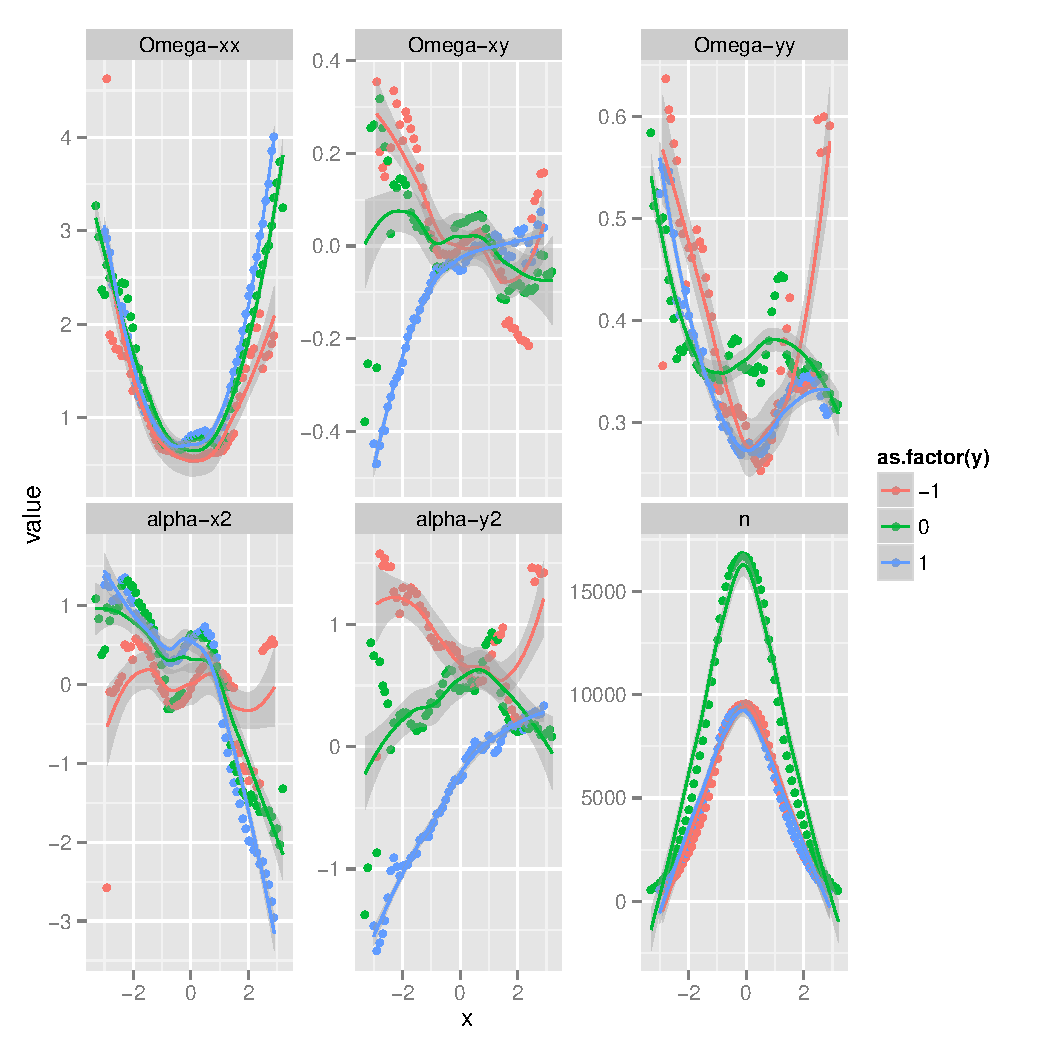
\includegraphics[width=10cm]{../scripts/flow/paramsChagingOverSpace.pdf}
\caption{Multivariate skew-normal parameters over space.}
\label{fig:smParamsOverSpace}
\end{figure}

\subsubsection{Results}


\subsubsection{Discussion}



\subsection{Coarse-to-fine}

People make shorter saccades over time. Include $1/f$ dynamics? 

\subsection{Left v Right}

Initially more fixations to the left half of the image \citep{nuthmann-matthias2014}.

\section{Using Biases for Better Analysis}

We will use the the central bias \citep{clarke-tatler2014} and \textit{saccadic flow} in some different contexts to see what biases can do for vision research. :p


\subsection{Attentional Landscapes}

Or do we call them hotspot maps?

\subsection{ROC Analysis}

Example of using our models rather than shuffle approaches.

\subsection{Flow and Coarse to fine}
To what extent does saccadic flow account for coarse-to-fine dynamics

\subsection{Inverse Yarbus}

Do these biases allow us to improve inverse yarbus performance?

\subsection{Salience}

Does salience explain the less likely saccades? 

\section{Discussion}

\section*{Acknowledgements}

Thanks to Adelchi Azzalini for advice on using the \texttt{sn} package for \texttt{R}. And mention grants. 

\bibliographystyle{plainnat}
\small
\bibliography{literature}
\end{document}